\chapter{Mapeamento Sistemático da Literatura}

\section{Objetivo e questões de pesquisa}

As pesquisas conduzidas nos repositórios de trabalhos, com base nas \textit{strings} de busca apresentadas na Tabela \ref{tab:keywords}, resultaram em 163 estudos após um processo de refinamento e testes iterativos das entradas. Esses trabalhos foram então categorizados e analisados em fases sequenciais, visando garantir uma revisão sistemática e abrangente.

\section{Resultados da Busca e Caracterização dos Estudos}

O processo de seleção, ilustrado na Figura \ref{fig:prisma_flowchart}, resultou na inclusão de 17 estudos para análise qualitativa.

\begin{figure}[H]
    \centering
    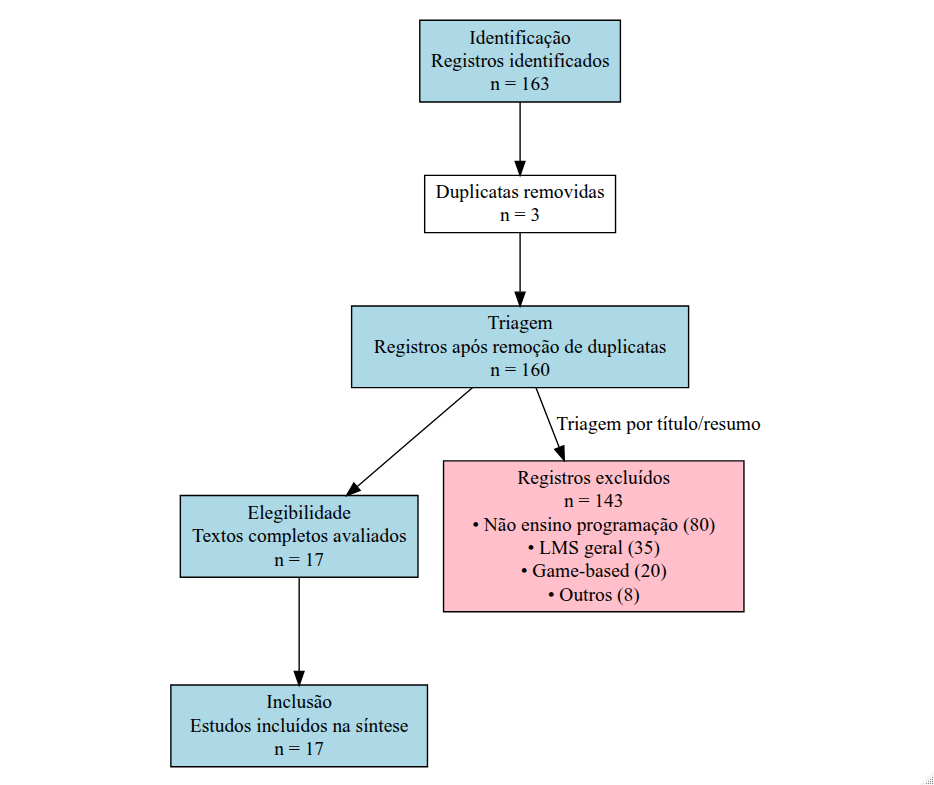
\includegraphics[width=1.1\linewidth]{../figuras/prisma-fluxograma.png}
    \caption{Fluxograma PRISMA do processo de seleção de estudos}
    \label{fig:prisma_flowchart}
\end{figure}

A Tabela \ref{tab:caracteristicas} sumariza as principais características destes estudos.

\begin{table}[h!]
\centering
\small
\begin{tabular}{|p{3cm}|p{2cm}|p{3cm}|p{4cm}|}
\hline
\textbf{Estudo} & \textbf{Ano} & \textbf{Foco Principal} & \textbf{Tipo de Log} \\
\hline
Arabyarmohamady et al. & 2012 & Detecção de plágio & Estilo de codificação \\
\hline
Annamaa & 2015 & IDE educacional & Logs de sessão Python \\
\hline
Raabe et al. & 2005 & Dificuldades de aprendizagem & Ambiente educacional \\
\hline
Liu et al. & 2018 & Comportamento do usuário & Logs de execução \\
\hline
Umezawa et al. & 2020 & Análise de erros lógicos & Histórico de arquivos \\
\hline
Pereira et al. & 2020 & Comportamento estudantil & Logs de IDE + Online Judge \\
\hline
Gu et al. & 2022 & Práticas de logging & Revisão sistemática \\
\hline
Silva et al. & 2022 & Predição de dificuldade & Métricas de código \\
\hline
Mangaroska et al. & 2022 & Estados cognitivos & Logs Eclipse + multimodal \\
\hline
Da Silva & 2022 & Análise de comunidades & Comportamento online \\
\hline
Nguyen et al. & 2023 & Avaliação automática & Git logs + qualidade \\
\hline
Educomp & 2023 & Complexidade vs dificuldade & Métricas de exercícios \\
\hline
Gupta et al. & 2024 & Padrões de programação & Clickstream data \\
\hline
Arguson et al. & 2022 & Erros de compilação & Logs de compilação \\
\hline
Liz-Domínguez et al. & 2022 & Desempenho acadêmico & Logs de LMS \\
\hline
Yang et al. & 2021 & Uso de logs na indústria & Práticas profissionais \\
\hline
Cândido et al. & 2021 & Monitoramento baseado em logs & Revisão sistemática \\
\hline
\end{tabular}
\caption{Características dos 17 estudos incluídos na síntese qualitativa}
\label{tab:caracteristicas}
\end{table}

\subsection{Perfil dos Estudos Incluídos} \label{subsec:perfis}
\begin{figure}
    \centering
    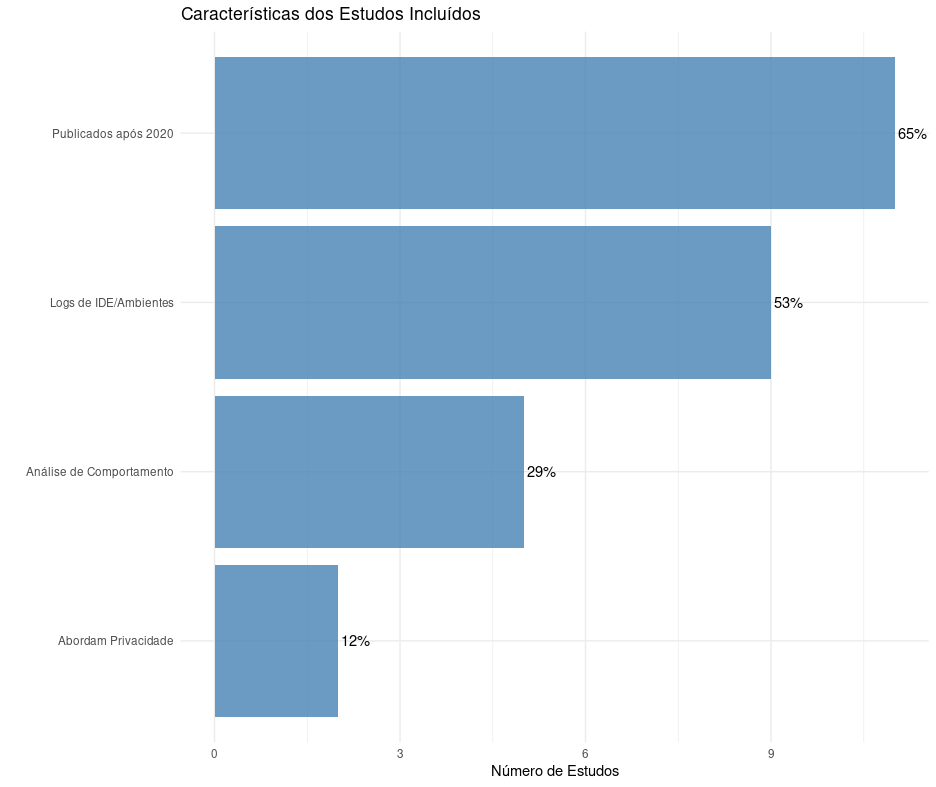
\includegraphics[width=0.75\linewidth]{../figuras/caracteristicas.png}
    \caption{Distribuição das características principais dos estudos incluídos (n=17)}
    \label{fig:placeholder}
\end{figure}

A análise dos 17 estudos revela um interesse crescente na área, com 65\% das publicações concentradas após 2020. A maioria dos estudos (53\%) utiliza logs de IDEs ou ambientes específicos, enquanto apenas 12\% abordam aspectos de privacidade e ética.

A análise temporal confirma o interesse crescente na área, com predominância de estudos recentes. Quanto ao foco metodológico, mais da metade utiliza logs de ambientes específicos, enquanto aspectos de privacidade permanecem pouco explorados.

\subsection{Respostas para QP1: Quais são os principais objetivos e aplicações do uso de logs no ensino de programação?} \label{subsec:respostas-qp1}

Os objetivos identificados foram categorizados em quatro áreas principais:

\begin{itemize}
    \item \textbf{Detecção de Dificuldades} (6 estudos): Umezawa (2020), Pereira (2020), Silva (2022), Educomp (2023), Arguson (2022), Raabe (2005)
    \item \textbf{Análise de Comportamento} (5 estudos): Gupta (2024), Liu (2018), Mangaroska (2022), Da Silva (2022), Liz-Domínguez (2022)
    \item \textbf{Qualidade de Código} (3 estudos): Arabyarmohamady (2012), Nguyen (2023), Annamaa (2015)
    \item \textbf{Práticas e Ferramentas} (3 estudos): Gu (2022), Yang (2021), Cândido (2021)
\end{itemize}

De acordo com \cite{gu2022logging}, ``A obtenção de logs é um processo que deve ser guiado por quatro questões fundamentais, conhecidas como 3W1H:

\begin{itemize}
    \item Why (Por quê): Qual é o objetivo da coleta de logs?
    \item Where (Onde): Em quais partes do sistema ou código os logs devem ser coletados?
    \item What (O que): Quais informações ou eventos devem ser registrados nos logs?
    \item How (Como): De que forma os logs serão coletados, armazenados e analisados?
\end{itemize}

Essas questões são essenciais para garantir que a geração de logs seja eficiente, relevante e alinhada aos objetivos do projeto, seja no desenvolvimento de software ou no contexto educacional. No ensino de programação, por exemplo, a aplicação do 3W1H pode ajudar a definir métricas e técnicas para monitorar o progresso dos estudantes e identificar dificuldades de aprendizado.

A abordagem feita por \cite{silva2022previsao} busca ``prever indicadores de dificuldade de exercícios de programação a partir de métricas de complexidade do código dos instrutores. Identificando registros de logs de JOs e relacionando esforço e dificuldade dos estudantes durante o desenvolvimento do código de solução''.

De acordo com \cite{gupta2024identification}, ``os dados de cliques (clickstream) e logs de atividades dos estudantes em plataformas de programação podem ser processados para extrair informações relevantes, como padrões de programação e relações entre características do código e o desempenho dos alunos. Essa análise permite que os instrutores identifiquem previamente estudantes com dificuldades ou baixo desempenho, ajustando suas metodologias de ensino e oferecendo suporte direcionado. Além disso, ao acompanhar a evolução do estilo de codificação dos alunos, os educadores podem avaliar a eficácia de suas estratégias pedagógicas e garantir que nenhum estudante seja deixado para trás em um mundo tecnologicamente avançado''.

O ensino de programação vai além da transmissão de conhecimentos técnicos, incluindo orientações sobre licenciamento de códigos e boas práticas de desenvolvimento. Nesse contexto, o combate ao plágio é uma preocupação relevante, e os logs surgem como uma ferramenta valiosa para apoiar a avaliação dos estudantes. Como argumenta \cite{arabyarmohamady2012coding}, características extraídas de cada código, como o estilo de programação, são armazenadas em um histórico (user profile). Esses dados permitem identificar mudanças no estilo de codificação e detectar se um código foi realmente desenvolvido pelo autor declarado ou se foi escrito por outra pessoa com um estilo diferente. Dessa forma, os logs não apenas auxiliam na identificação de plágio, mas também contribuem para uma avaliação mais precisa e personalizada do aprendizado dos estudantes.

Outra aplicação relevante para a geração de logs é a criação de \textit{datasets}, como demonstrado no trabalho de \cite{umezawa2020analysis}. O estudo detecta diversos elementos em códigos-fonte, como declarações de variáveis, funções, estruturas condicionais, laços de repetição, operações de leitura e escrita, espaçamento, pontuação, expressões lógicas e matemáticas, além de comentários. Esses dados são organizados em tabelas para análise. Um exemplo interessante é o uso do espaçamento: embora não afete a execução do código, padrões de espaçamento 'incorretos' ou idênticos podem indicar que vários estudantes estão cometendo o mesmo erro ou copiando trechos de código uns dos outros. Isso demonstra que os logs vão além da identificação de erros de lógica ou sintaxe, podendo revelar padrões de comportamento e práticas comuns entre os estudantes. Além disso, o trabalho destaca a importância de estruturas de controle, como declarações 'for' e 'if', e a frequência de alterações em variáveis e números, que refletem a natureza repetitiva dos exercícios universitários. Esses insights mostram o potencial dos logs para apoiar educadores na identificação de dificuldades e na melhoria do ensino de programação.

\subsection{Respostas para QP2: Quais ferramentas, métodos e métricas são mais utilizados para capturar, armazenar e analisar logs em ambientes de ensino de programação?} \label{respostas-qp2}

No trabalho de \cite{pereira2020using}, foi desenvolvida uma IDE para obter todas as informações. ``O CodeBench fornece o seu próprio editor de código (IDE), concebido para ser simples e fácil de utilizar por principiantes. Todas as ações executadas pelos alunos no IDE (por exemplo, teclas digitadas, submissões, colagem de código, cliques do mouse, transições de separadores ou de janelas, etc.) são registradas e gravadas em arquivos de registro no lado do servidor.''

Para \cite{liu2018user}, ``Cada evento representa o registro de uma chamada de método durante a execução do software. Portanto, todos os eventos podem ser alinhados com padrões de comportamento previamente identificados. Ao utilizar um log de execução de software e os padrões de comportamento treinados como entrada, realizamos a correspondência baseada em alinhamento (alignment-based matching) para obter um log abstrato de operações do usuário.'' Essa técnica pode ser aplicada no ensino de programação para analisar as interações dos estudantes com ferramentas de desenvolvimento, identificar erros comuns e fornecer feedback personalizado com base em seu comportamento durante a codificação.

O trabalho de \cite{mangaroska_exploring_2022} utiliza algumas ferramentas para capturar a interação do usuário, contudo, na questão de logs, foi utilizada uma extensão para o Eclipse e foi definida assim: ``Log data: Um plugin para Eclipse que possui uma aba, visualização (Trætteberg et al., 2016), foi utilizado para obter comportamentos de leitura e escrita dos estudantes. Este plugin armazena o estado do programa toda vez que o estudante salva o programa, usando o atalho ou botão de salvar.''

A ferramenta desenvolvida por \cite{annamaa2015thonny}, uma IDE projetada na Universidade de Tartu com interface amigável para iniciantes em Python, coleta informações detalhadas sobre cada sessão de programação. Esses dados incluem eventos como carregar, salvar e modificar arquivos, além de diferenciar textos copiados de textos digitados. As informações coletadas permitem reproduzir todo o processo de construção do programa e as atividades realizadas no shell. Para isso, a ferramenta oferece uma janela separada onde o usuário pode selecionar um arquivo de log e visualizar a reprodução dos eventos em velocidade ajustável. Essa funcionalidade é particularmente útil para educadores, pois permite analisar o processo de desenvolvimento dos estudantes e identificar possíveis dificuldades.

Nos últimos anos, a educação em programação tem passado por uma transformação significativa com a introdução de Sistemas Automatizados de Avaliação de Programação (APASs). Esses sistemas revolucionaram a forma como as tarefas de programação são avaliadas, oferecendo vantagens tanto para educadores quanto para estudantes. O ProgEdu, desenvolvido por \cite{nguyen_analyzing_2023}, é um exemplo de aplicação baseada na web que combina as funcionalidades de um Sistema de Gestão de Aprendizagem (LMS) com um APAS. A ferramenta permite que os estudantes acessem atividades, submetam códigos e recebam feedback automatizado, facilitando a identificação de erros e o aprimoramento das habilidades de programação. Além disso, o ProgEdu é uma aplicação baseada em Docker, o que garante portabilidade e facilidade de implantação. A automação do processo de avaliação não apenas reduz a carga de trabalho dos instrutores, mas também oferece avaliações consistentes e imparciais, aplicando critérios predefinidos de forma objetiva. Essa abordagem é particularmente relevante no contexto da Educação a Distância (EAD), onde a popularização de serviços baseados na web tem se tornado cada vez mais comum.

\section{Identificação dos Estudos} \label{sec:identificacao-estudos}
\subsection{Estratégia de Busca} \label{subsec:estrategias-buscas}
A pesquisa foi realizada em cinco bibliotecas virtuais, utilizando como critérios de busca palavras-chave e \textit{strings} de busca com operadores lógicos \textit{AND} e \textit{OR}. Os repositórios de pesquisa utilizados são apresentados na Tabela \ref{tab:repositorios}.

\begin{table}[h!]
\centering
\small
\begin{tabular}{|m{3cm}|m{5cm}|}
\hline 
\textbf{Repositório} & \textbf{Resultados} \\ 
\hline 
Scopus & 23 \\ 
\hline 
IEEE Xplore & 2 \\ 
\hline 
SOL SBC & 2 \\ 
\hline 
ACM & 127 \\
\hline
WILEY & 9 \\ 
\hline
\end{tabular}
\caption{Lista de repositórios de pesquisa utilizados no estudo.}
\label{tab:repositorios}
\end{table}

As combinações de palavras-chave e operadores utilizadas na pesquisa são apresentadas na Tabela \ref{tab:keywords}.

\begin{table}[h!]
\centering
\footnotesize
\begin{tabular}{|p{16cm}|}
\hline 
\multicolumn{1}{|c|}{\textbf{Palavras-chave e Operadores}} \\ 
\hline 
programming AND teaching AND log AND NOT (log-based) AND NOT (metrics) AND systematic AND review \\ 
\hline 
programming AND teaching AND log AND NOT (log-based) AND (integrate AND development AND environment) AND NOT (visual AND programming) AND NOT (web AND application) \\ 
\hline 
telemetry AND education AND programming AND log \\ 
\hline 
ontology AND education AND programming AND log AND dataset \\
\hline
artefact AND cognitive AND learning \\
\hline
background AND teaching AND log AND NOT (log-based) AND (systematic AND review) \\
\hline
log AND (``teaching programming" OR ``learning programming") AND (``IDE" OR ``integrated development environment")) NOT (``log-based" OR ``lms" OR ``learning management system" \\ 
\hline
(log AND ("teaching programming" OR "learning programming") AND ("IDE" OR "integrated development environment")) NOT ("log-based" OR "lms" OR "learning management system" OR "game-based" OR "game based" OR "gamification") \\ 
\hline
\end{tabular}
\caption{Combinações de palavras-chave e operadores utilizados na pesquisa.}
\label{tab:keywords}
\end{table}

\subsection{Idioma dos Trabalhos}\label{sub:idioma-trabalhos}
Os trabalhos foram selecionados em português e inglês. A inclusão do português justifica-se pela relevância de pesquisas nacionais, especialmente no contexto das Instituições de Ensino Federais brasileiras. O inglês, por sua vez, foi escolhido por ser o idioma predominante em publicações acadêmicas internacionais, como conferências e periódicos de alto impacto.

\subsection{Critérios de Inclusão}\label{sub:criterios-inclusao}
\label{inclusion-critery}
Após a execução das buscas utilizando as \textit{strings} definidas, os artigos identificados foram submetidos a um processo de triagem. Foram adotados os seguintes critérios para inclusão:

\begin{enumerate}
    \item Relevância temática: O artigo deve abordar explicitamente o uso de logs no ensino de programação, conforme verificado pela análise de títulos e resumos.
    \item Revisão sistemática: Trabalhos que se caracterizam como revisões sistemáticas da literatura também foram incluídos, devido à sua contribuição para a compreensão do estado da arte no tema.
\end{enumerate}

\subsection{Critérios de Exclusão}\label{sub:criterios-exclusao}
Foram excluídos textos que, mesmo contendo a \textit{string} de busca, retornaram resultados relacionados a:

\begin{enumerate}
    \item \textit{Log-based}: abordagens ou técnicas que utilizam logs como base principal (por exemplo, sistemas de monitoramento ou análise de logs).
    \item Uso de logs em outras áreas da educação: aplicações de logs em contextos educacionais que não envolvem diretamente o ensino de programação.
    \item \textit{Learning Management Systems (LMS)}: trabalhos que abordam o uso de logs em plataformas de gestão de aprendizagem (LMS), como Moodle, Canvas ou Blackboard, sem foco específico no ensino de programação.
    \item \textit{Game-based learning}: trabalhos que utilizam jogos ou mecânicas de jogos como principal estratégia de ensino, sem foco no uso de logs para análise de aprendizagem.
\end{enumerate}

\section{Lacunas Identificadas e Trabalhos Futuros}\label{sec:lacunas-identificadas}

A análise revelou lacunas significativas:
\begin{itemize}
    \item \textbf{Padronização}: Ausência de modelos comuns para logs educacionais
    \item \textbf{Privacidade}: Poucos estudos abordam aspectos éticos
    \item \textbf{Contexto Brasileiro}: Limitada pesquisa em instituições brasileiras
\end{itemize}